\section{Results}
\label{sec:results}

\subsection{Behavioral Evaluation}
\label{sec:behavioral}

\Tabref{tab:behavioral} reports the behavioral accuracy of \gptsmall on each task. The model performs at or below chance on all three tasks: it essentially random-guesses on comparison (48.6\% vs.\ 50\% chance), matches the majority-class baseline on interval membership (72.9\%, identical to the ``always No'' rate), and completely fails on ring counting (0.0\% vs.\ 3.8\% chance). These results confirm that \gptsmall was not trained to solve these tasks in our prompt format, establishing a baseline against which internal representations can be contrasted.

\begin{table}[t]
\centering
\caption{Behavioral accuracy of \gptsmall on each task. The model performs at or below chance on all tasks, establishing that any information recovered by probing reflects internal representations that are not surfaced in the model's outputs.}
\label{tab:behavioral}
\begin{tabular}{@{}lcc@{}}
\toprule
\textbf{Task} & \textbf{Accuracy (\%)} & \textbf{Chance (\%)} \\
\midrule
Number Comparison ($A > B$?) & 48.6 & 50.0 \\
Interval Membership ($X \in [A,B]$?) & 72.9 & 72.9 \\
Ring Counting (mod 26) & 0.0 & 3.8 \\
\bottomrule
\end{tabular}
\end{table}

\subsection{Linear Probing: Comparison and Interval}
\label{sec:probing_results}

\Figref{fig:probing} and \tabref{tab:probing} present probe accuracy across layers for comparison and interval membership. Two patterns emerge.

\para{Comparison information is nearly perfectly decodable.} Probe accuracy jumps from chance (51.4\%) at the embedding layer to 89.4\% at layer~1, then rises steadily to a peak of \textbf{99.1\%} at layer~9. Shuffled-label controls remain at 51--54\% throughout, confirming that the probe extracts genuine task-relevant structure. This 99.1\% accuracy---despite 48.6\% behavioral accuracy---constitutes a 50.5 percentage point gap between internal representation and behavioral performance.

\para{Interval membership is harder but still well-represented.} Interval probe accuracy rises from the majority-class baseline (72.9\%) at layer~0 to a peak of \textbf{83.8\%} at layer~8, then declines slightly in later layers. The gap above shuffled controls (83.8\% vs.\ 62.5\% at layer~8) is 21.3 percentage points. The 15 percentage point gap between comparison (99.1\%) and interval (83.8\%) peak accuracy is consistent with the hypothesis that interval membership requires composing two boundary checks.

\begin{table}[t]
\centering
\caption{Linear probe accuracy (\%) by layer for comparison and interval membership tasks. We report both real-label and shuffled-label (control) accuracy. Best real-label results are in \textbf{bold}.}
\label{tab:probing}
\resizebox{\textwidth}{!}{
\begin{tabular}{@{}lcccccccccccccc@{}}
\toprule
& & \multicolumn{13}{c}{\textbf{Layer}} \\
\cmidrule(lr){3-15}
\textbf{Task} & \textbf{Labels} & 0 & 1 & 2 & 3 & 4 & 5 & 6 & 7 & 8 & 9 & 10 & 11 & 12 \\
\midrule
Comparison & Real & 51.4 & 89.4 & 92.1 & 94.0 & 95.0 & 94.6 & 98.5 & 98.9 & 99.0 & \textbf{99.1} & 98.9 & 98.4 & 97.6 \\
Comparison & Shuffled & 51.4 & 53.9 & 54.2 & 51.4 & 50.4 & 52.0 & 52.5 & 52.5 & 53.1 & 52.7 & 53.1 & 51.9 & 53.7 \\
\midrule
Interval & Real & 72.9 & 73.7 & 73.1 & 77.9 & 79.4 & 80.4 & 81.4 & 82.9 & \textbf{83.8} & 82.1 & 80.5 & 81.5 & 81.9 \\
Interval & Shuffled & 72.9 & 59.2 & 57.7 & 58.7 & 60.5 & 61.3 & 61.3 & 61.4 & 62.5 & 63.2 & 64.5 & 65.4 & 63.8 \\
\bottomrule
\end{tabular}
}
\end{table}

\begin{figure}[t]
\centering
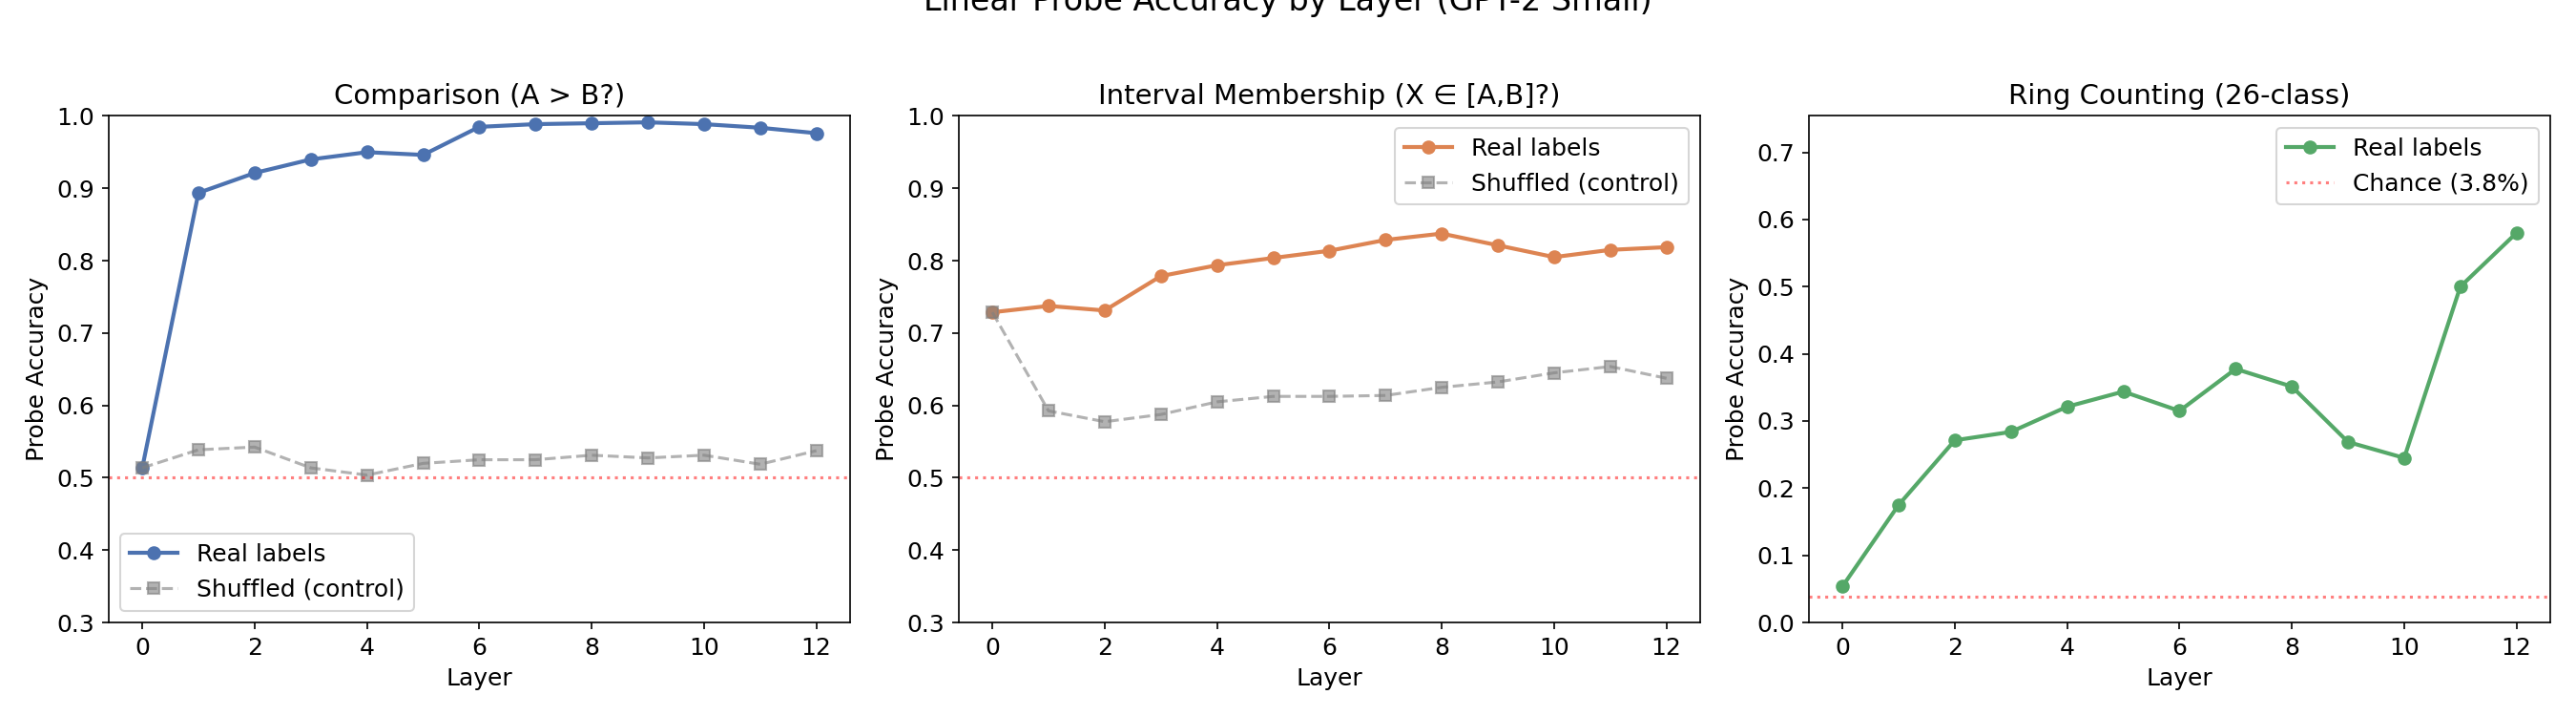
\includegraphics[width=0.95\linewidth]{figures/probing_by_layer.png}
\caption{Probe accuracy by layer for comparison and interval membership tasks, with shuffled-label controls. Comparison information is nearly perfectly decodable by layer~9 (99.1\%), while interval membership peaks at 83.8\% at layer~8. Both are far above their respective shuffled-label baselines.}
\label{fig:probing}
\end{figure}

\subsection{Linear Probing: Ring Counting}
\label{sec:ring_results}

\Tabref{tab:ring} reports probe accuracy for the 26-class ring counting task. Despite 0\% behavioral accuracy, the linear probe achieves \textbf{58.0\%} accuracy at layer~12---15$\times$ the 3.8\% chance level. Accuracy increases monotonically from 5.4\% at the embedding layer to 58.0\% at the final layer, with the steepest gains in layers~1--3 and 9--12. This progressive buildup mirrors the pattern observed by \citet{hasani2026mechanistic} for counting, but extends it to modular arithmetic.

\para{Wrap-around hurts accuracy.} We split examples by whether they require wrapping past Z. No-wrap examples are consistently easier to decode (64.0\% vs.\ 55.4\% at layer~12), a gap of 5--9 percentage points across layers. This confirms that modular arithmetic adds computational complexity beyond simple addition.

\begin{table}[t]
\centering
\caption{Ring counting probe accuracy (\%) by layer for all examples and split by wrap condition. Chance level is 3.8\% (1/26). Best results in \textbf{bold}.}
\label{tab:ring}
\begin{tabular}{@{}lccc@{}}
\toprule
\textbf{Layer} & \textbf{All} & \textbf{No-Wrap ($n{=}414$)} & \textbf{Wrap ($n{=}386$)} \\
\midrule
0 (embed) & 5.4 & 7.2 & 9.6 \\
1 & 17.5 & -- & -- \\
3 & 28.4 & 60.4 & 52.8 \\
6 & 31.5 & 59.4 & 53.4 \\
9 & 26.9 & 54.3 & 46.9 \\
11 & 50.0 & -- & -- \\
12 & \textbf{58.0} & \textbf{64.0} & \textbf{55.4} \\
\bottomrule
\end{tabular}
\end{table}

\subsection{Regression Probing: Numerical Value Decoding}
\label{sec:regression}

Ridge regression probes achieve near-perfect decoding of numerical values from layer~1 onward (\figref{fig:regression}). For the query value $X$ in interval prompts, $R^2$ reaches 0.992 at layer~1 and 0.999 at layer~12. For the offset $N$ in ring counting prompts, $R^2$ is effectively 1.000 from layer~1 onward. These results confirm prior findings~\citep{levy2024language} that transformers faithfully encode numerical values in their residual streams, and show that this encoding is available from the earliest transformer layers.

\begin{figure}[t]
\centering
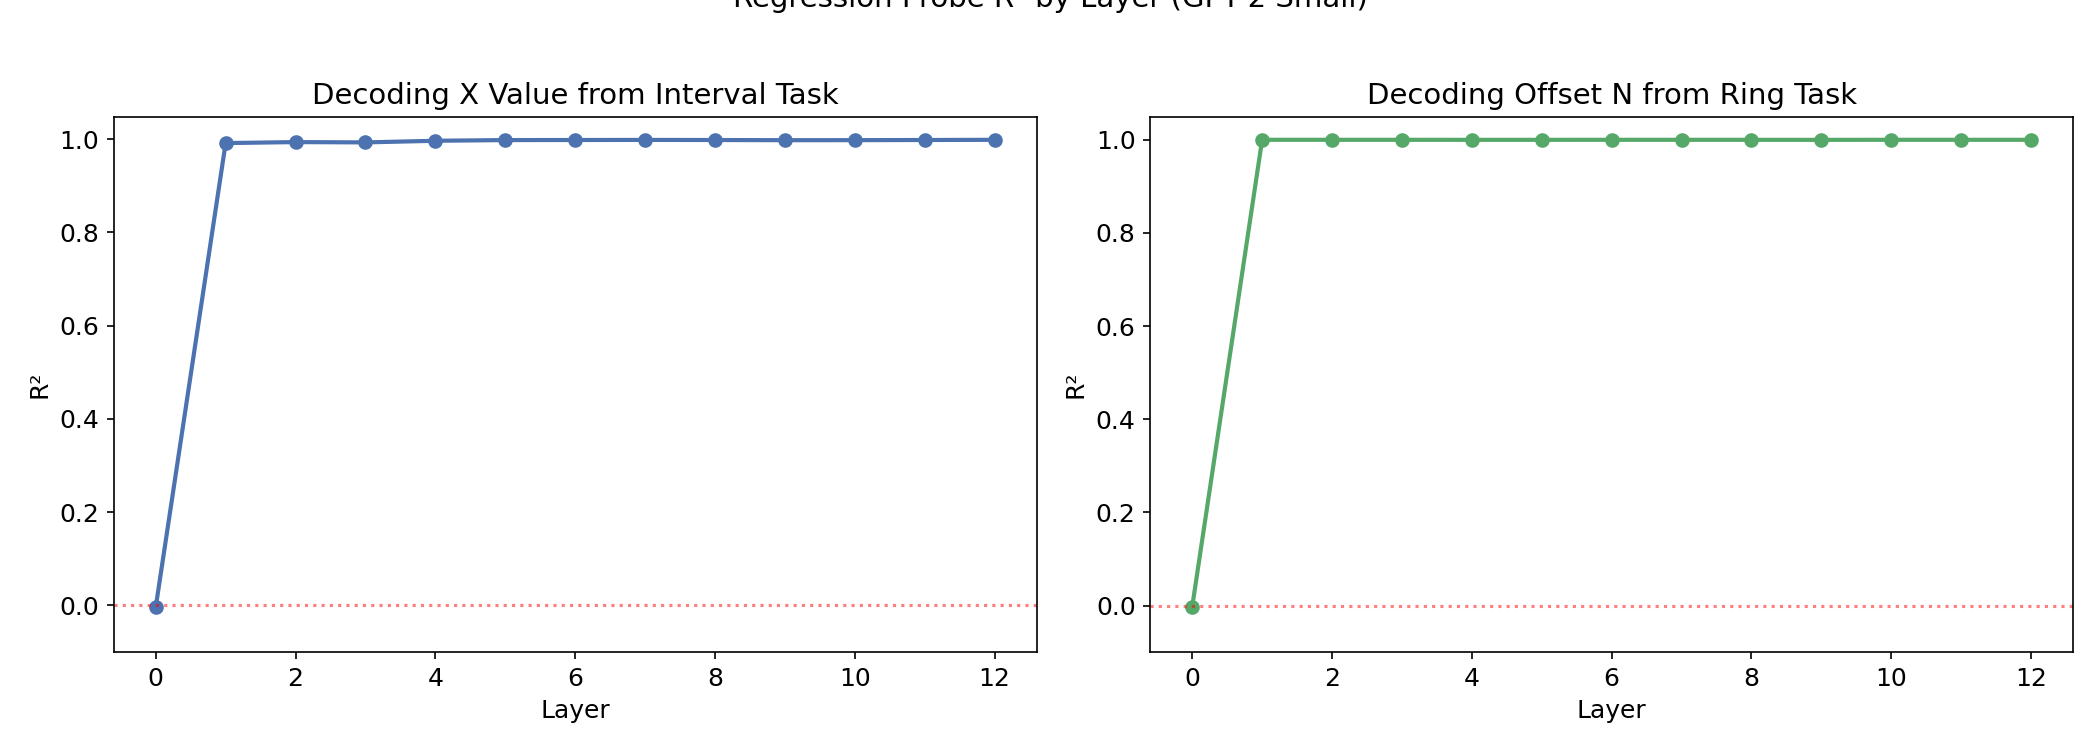
\includegraphics[width=0.65\linewidth]{figures/regression_probing.png}
\caption{Regression probe $R^2$ by layer for decoding numerical values ($X$ from interval prompts, $N$ from ring counting prompts). Both values are near-perfectly decodable ($R^2 > 0.99$) from layer~1 onward.}
\label{fig:regression}
\end{figure}

\subsection{Interval Membership by Width}
\label{sec:width}

\Tabref{tab:width} and \figref{fig:width} present probe accuracy stratified by interval width. Narrow intervals (width 2, 5) show high probe accuracy at all layers (93--99\%), but this is largely driven by class imbalance: with only 1--6.5\% positive labels, a probe can achieve high accuracy by defaulting to ``No.'' For the most balanced condition (width 50, $\sim$50\% positive), probe accuracy rises from 50.5\% at layer~0 (chance) to \textbf{75.5\%} at layer~9, demonstrating genuine learning. Width~20 shows an intermediate pattern, with accuracy improving from 77.0\% to 84.0\% at layer~9.

\begin{table}[t]
\centering
\caption{Interval membership probe accuracy (\%) by interval width and layer. Narrow intervals (width 2, 5) have highly imbalanced labels, inflating accuracy. Width~50 provides the most informative comparison. Best per-width results in \textbf{bold}.}
\label{tab:width}
\begin{tabular}{@{}lccccc@{}}
\toprule
\textbf{Layer} & \textbf{Width 2} & \textbf{Width 5} & \textbf{Width 10} & \textbf{Width 20} & \textbf{Width 50} \\
\midrule
0 (embed) & 99.0 & 93.5 & 92.5 & 77.0 & 50.5 \\
3 & 99.0 & 96.5 & 91.5 & 77.5 & 73.4 \\
6 & 99.0 & 95.0 & 92.0 & 77.5 & 71.0 \\
9 & 99.0 & 93.0 & 92.0 & \textbf{84.0} & \textbf{75.5} \\
12 & 99.0 & 93.0 & 91.5 & 78.0 & 70.5 \\
\bottomrule
\end{tabular}
\end{table}

\begin{figure}[t]
\centering
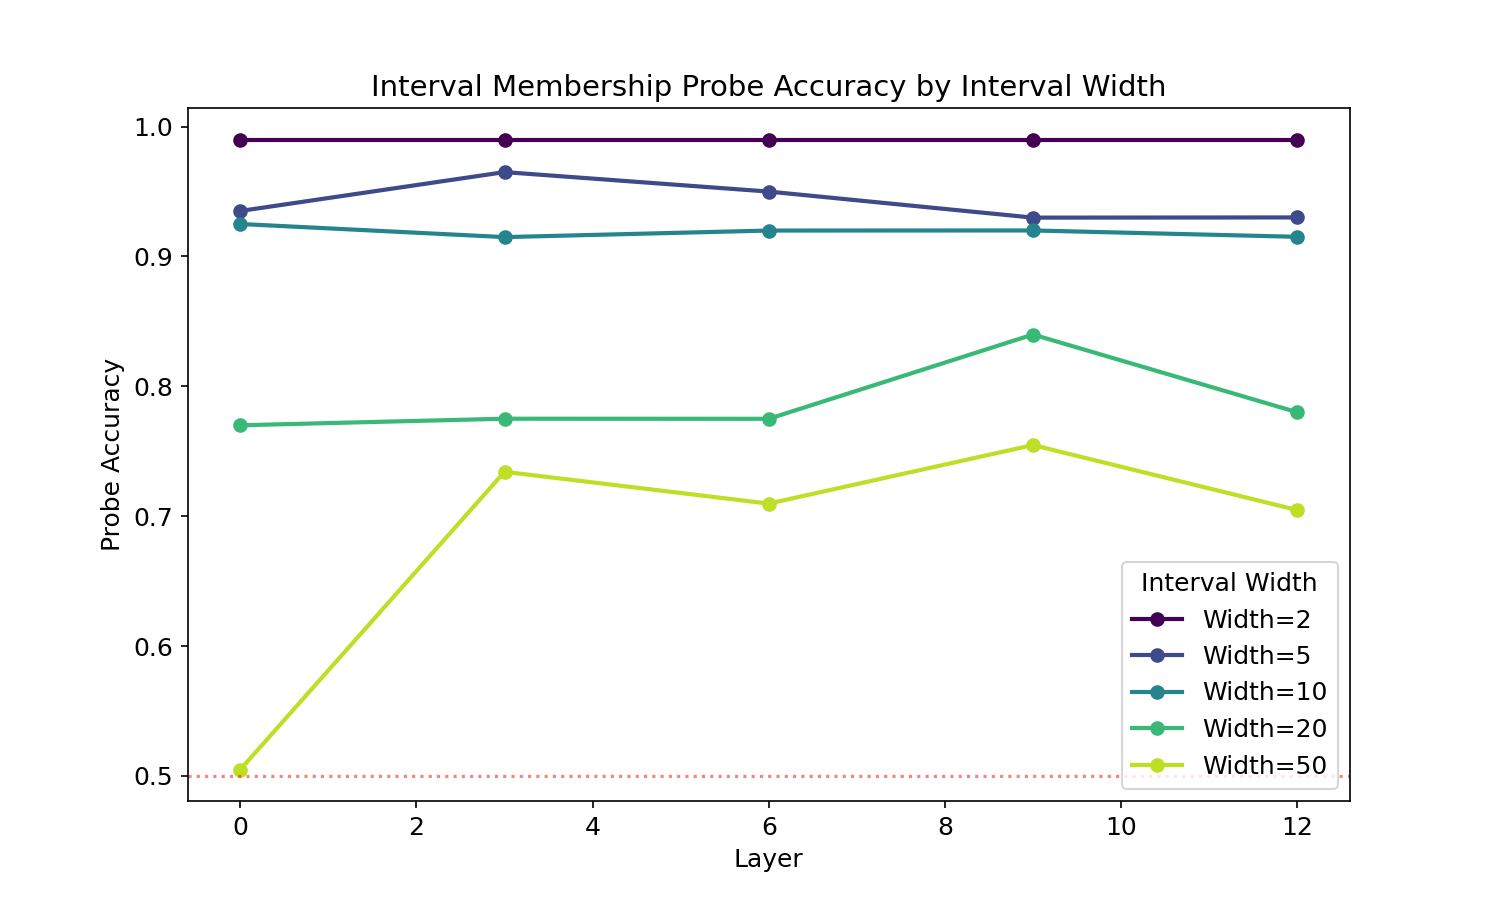
\includegraphics[width=0.65\linewidth]{figures/width_analysis.png}
\caption{Interval membership probe accuracy by width across layers. Narrow intervals (width 2, 5) achieve high accuracy trivially via class imbalance. Width~50 (approximately balanced) shows genuine improvement from chance at layer~0 to 75.5\% at layer~9.}
\label{fig:width}
\end{figure}

\subsection{Activation Patching}
\label{sec:patching_results}

\Figref{fig:patching} shows activation patching results for comparison and interval membership. For both tasks, patching effects are negligible in early layers (0--4), grow in magnitude through layers~5--7, and peak at layers~8--9. For comparison, the peak effect is $-0.087$ (layer~9); for interval membership, it is $-0.065$ (layer~9). The effects are \emph{negative}, meaning that patching from a positive-label source into a negative-label target moves the prediction further from ``Yes'' rather than toward it. This counterintuitive result is consistent with the model's near-chance behavioral accuracy: since the model is not reliably solving these tasks, patching does not transfer a coherent ``correct answer'' signal but instead introduces a perturbation. The high variance in later layers (standard deviations up to 0.22) further reflects this instability.

Despite the sign, the \emph{magnitude} profile is informative: layers~8--9 produce the largest perturbation effects for both tasks, consistent with \citet{hanna2023how}'s identification of layers~5--9 as the location of the greater-than circuit.

\begin{figure}[t]
\centering
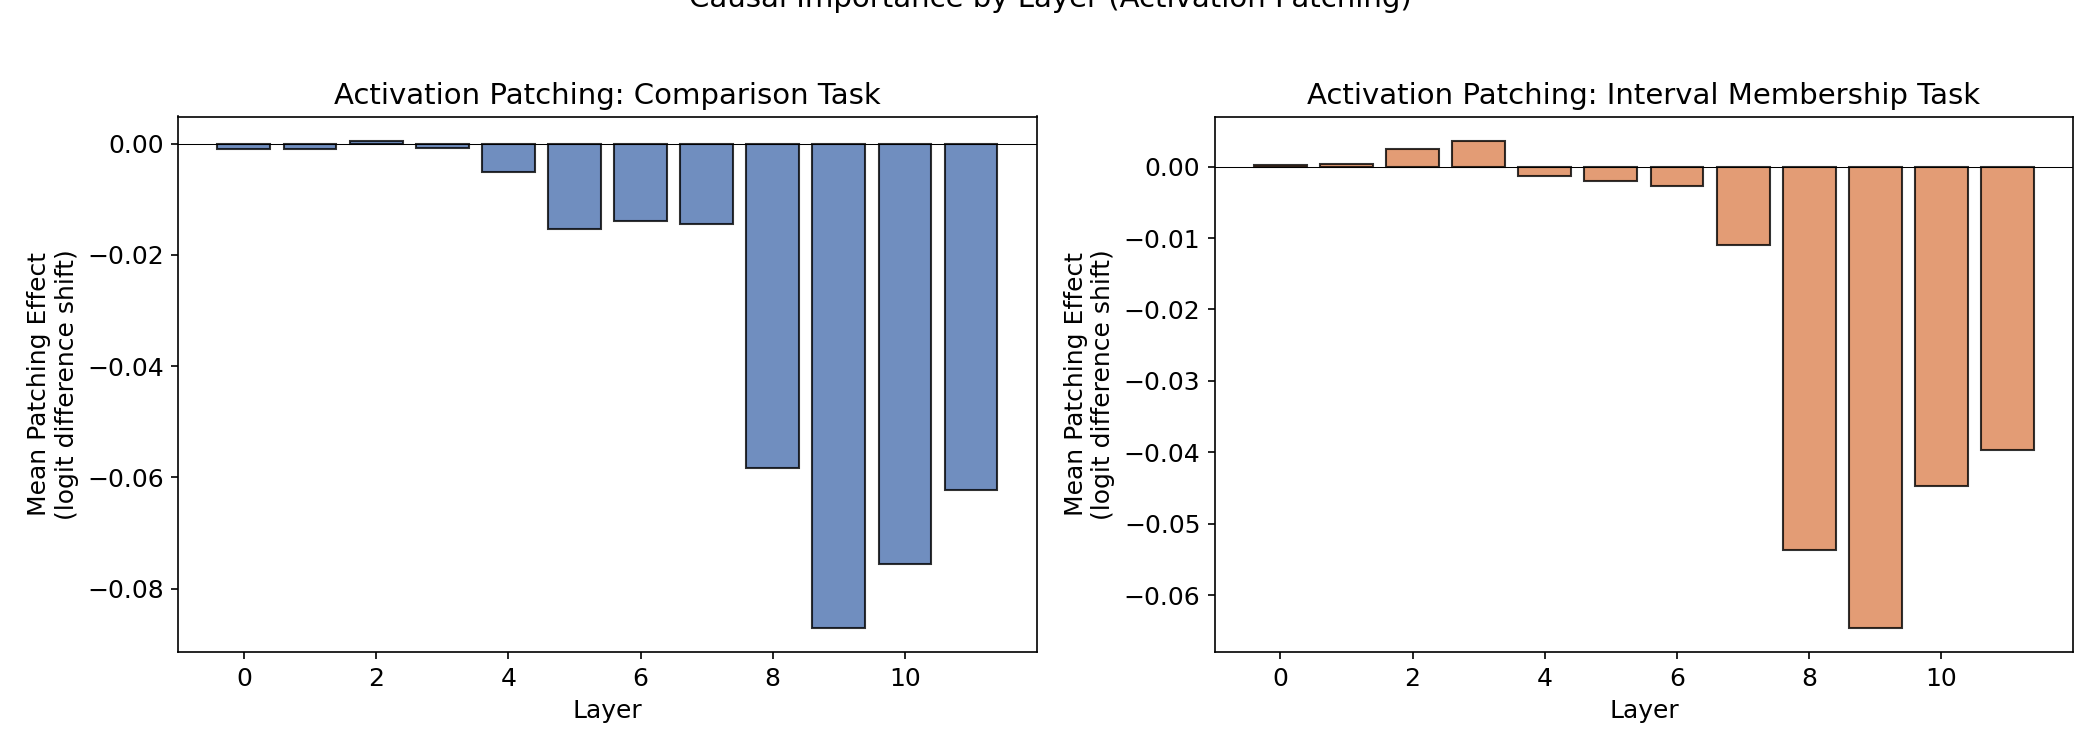
\includegraphics[width=0.65\linewidth]{figures/activation_patching.png}
\caption{Activation patching effects by layer for comparison and interval membership. Both tasks show peak perturbation at layers~8--9, consistent with prior work on the greater-than circuit location. Negative effects reflect the model's inability to reliably solve these tasks behaviorally.}
\label{fig:patching}
\end{figure}
